\section{Balsa workflow optimisation through STG resynthesis}

\label{sec:balsa-workflow}

\begin{figure}
\centering
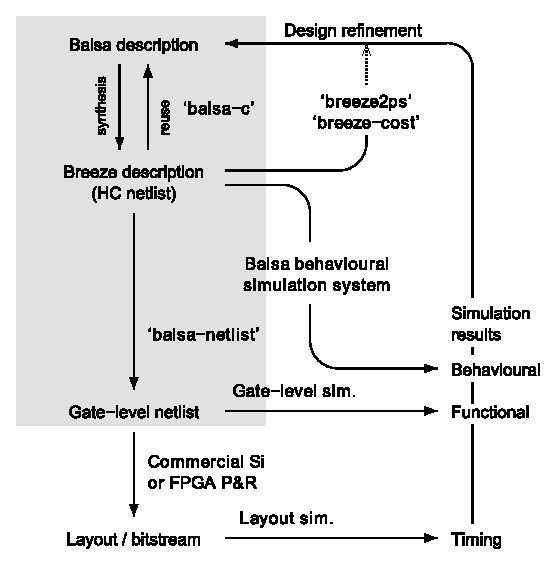
\includegraphics[width=0.40\paperwidth]{figures/balsa-design-workflow}

\caption{Balsa design workflow\label{fig:Balsa-design-workflow}}
\end{figure}


\begin{figure}
\centering
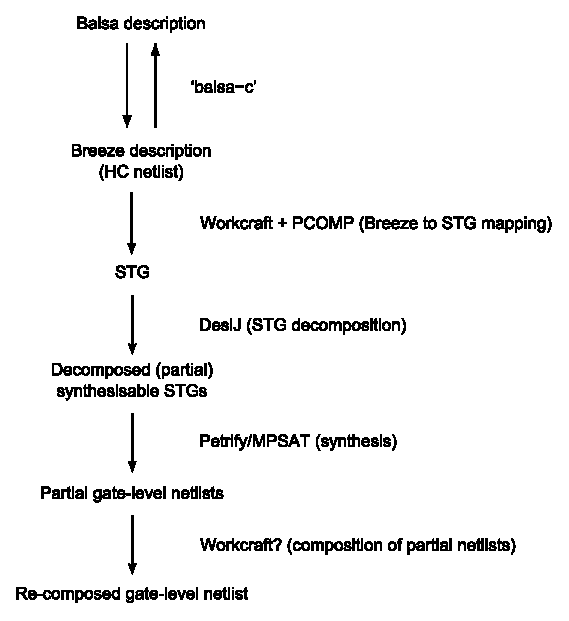
\includegraphics[width=0.40\paperwidth]{figures/balsa-workflow-modification}

\caption{Modified Balsa workflow\label{fig:Modified-Balsa-workflow}}
\end{figure}


The standard Balsa design workflow is comprised of several stages~(Figure~\ref{fig:Balsa-design-workflow}).
The designer writes the system specification in Balsa language. It
is passed to the Balsa compiler, which generates a handshake component
netlist (produced in a language called Breeze) using syntax-directed
mapping on the source code. Syntax-directed mapping in this context
means that there is a predefined handshake component construct for
every syntactic structure. The Breeze netlist is then translated into
a gate-level netlist using direct mapping, this time from individual
handshake components to their gate-level implementation, which is
defined beforehand.

The proposed modification of this workflow is shown in~Figure~\ref{fig:Modified-Balsa-workflow}.
The translation from Balsa language into Breeze netlist is retained
(and is still done by the Balsa compiler), but the Breeze-netlist
to gate-level-netlist mapping is replaced with the STG resynthesis
flow as introduced in section~\ref{sec:Balsa-Introduction}. Instead of
using Balsa tools to produce a gate-level netlist, the Breeze netlist
is read by a special interpreted graph model plug-in to \noun{Workcraft
}tool~\cite{DBLP:conf/apn/PoliakovKY09}, which replaces the handshake
components with their STG specifications and produces a composition
of those STGs using \noun{PComp} tool. If the resulting STG is small
enough, the gate-level implementation may immediately be synthesised
using any of the available synthesis tools.

However, for many practical cases the composed STG will become quite
large. In this case, to synthesise the implementation it is necessary
to insert an additional decomposition step, which may be either STG
decomposition~(implemented using a tool called \noun{DesiJ~}\cite{DesiJ}
that is automatically called from the plug-in), or\noun{ }handshake
circuit~(HC) decomposition which is supported by the plug-in directly.
Therefore, the whole process is automated in the \noun{Workcraft }framework.

The technique allows to synthesise more efficient control circuits
while at the same time preserving the benefit of rapid design methodology
fundamental to Balsa. It should be noted, however, that full modelling
of all Breeze components with STGs is not practical. The behaviour
of most data components would be too complex to synthesise from an
STG. Circuit resynthesis for such components would take too much time
and would often be less effective than an already existing gate-level
implementation done by an experienced designer. Subsequently, all
data-related functionality in HCs is modelled outside of STG composition
framework: the STG models include only control signals for the data
path elements. These control signals are to be connected after the
gate-level generation step to the data-path circuit that is assembled
separately (its components are specified by a structural Verilog netlist).
The data path is generated automatically side-by-side with the STG
behaviour model.


\subsection{Support of Breeze handshake circuits as interpreted graph model in
\noun{Workcraft}}

For the purpose of implementation of the design flow discussed in
this section the \noun{Workcraft} framework was extended with a plug-in
that introduces support for Breeze HCs. The new HC model allows \noun{Workcraft}'s
convenient visual editing tools to be applied for creation and editing
of Breeze netlists. The same plug-in also performs generation of the
STG behaviour model for the specified HC. The STG generation algorithm
is designed to be highly customisable, with support of multiple handshake
protocols and various STG implementations for each type of component.
At the moment of writing, STG generation was implemented for a limited
set of components using early 4-phase handshake protocol. The library
of components is being expanded and will include all Breeze components
with support for different handshake protocols.


\subsection{STG specifications of individual handshake components\label{sec:Individual-component-examples}}

Balsa components can be roughly divided in three groups: pure control
components, data path control components and data-control interface
components. We will review each group separately.


\subsubsection{Pure control path components}

\newcommand{\vcent}[1]{
  $\vcenter{\hbox{#1}}$
}
\newcommand{\balsafigSZ}[1]{
\vcent{\includegraphics[scale=0.6]{#1}}
}

\begin{figure}
\centering
\subfloat[Sequence\label{fig:SequenceOptimised}]{
\centering
\balsafigSZ{figures/Control/sequence-HC}
~~
\vcent{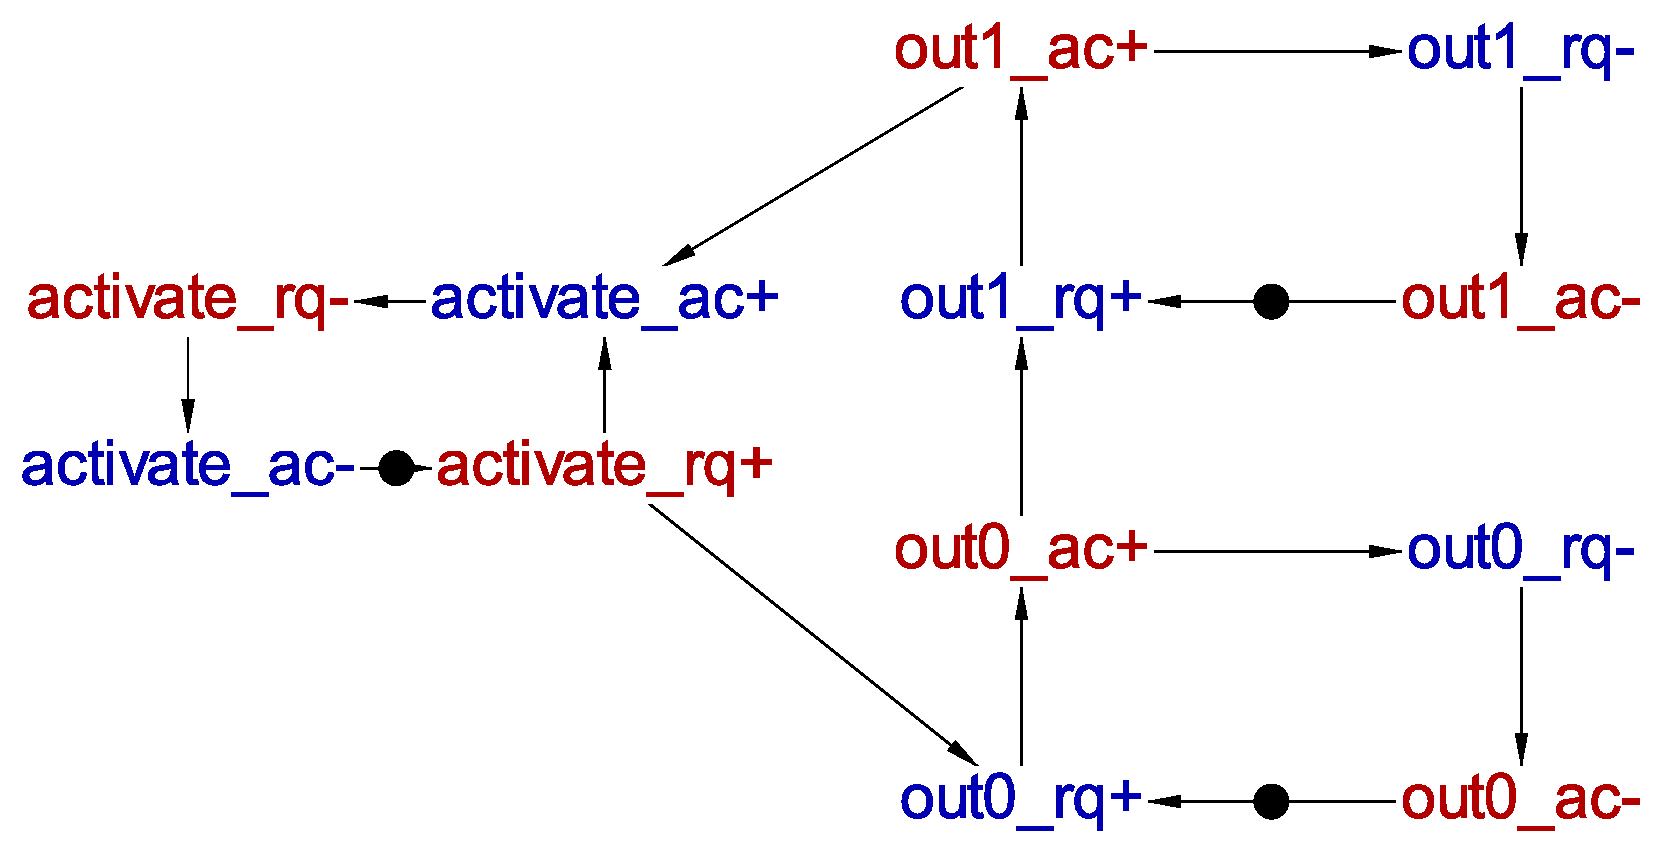
\includegraphics[scale=0.25]{figures/Control/sequenceoptimised}}
}

\subfloat[Concur\label{fig:Concur}]{
\centering
\balsafigSZ{figures/Control/concur-HC}~~\vcent{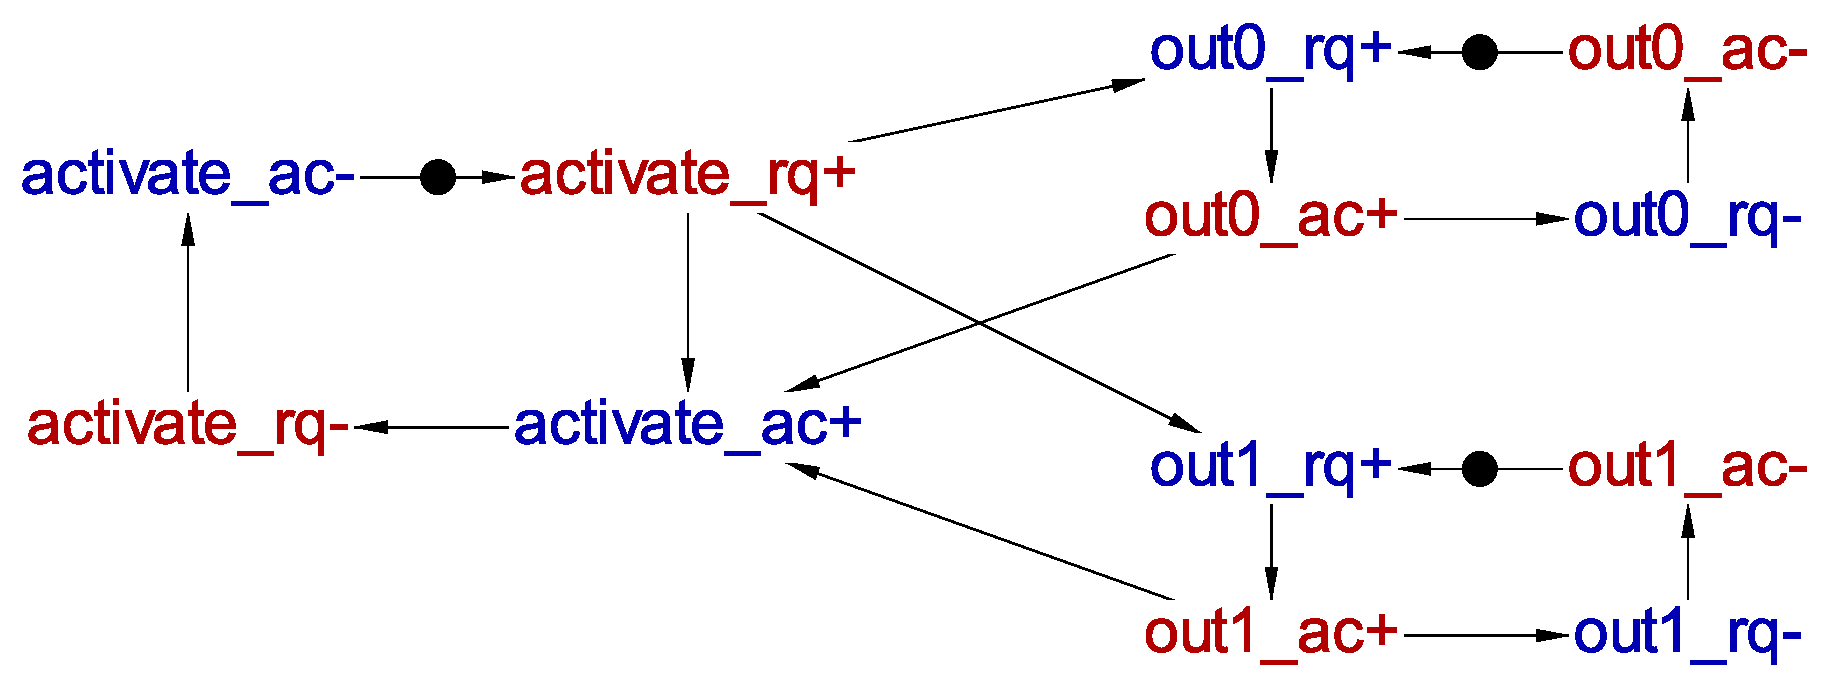
\includegraphics[scale=0.25]{figures/Control/concur}}
}

\caption{Pure control path handshake components and their respective STGs}
\end{figure}


Pure control components only control the behaviour of other components
and do not carry out any data operations. These components are expected
to gain the most from the new design workflow because all of their
handshakes are inside the control path and such handshaking does not
have to always strictly correspond to the general protocol.

The examples are Concur~(Figure~\ref{fig:Concur}) and SequenceOptimised~(Figure~\ref{fig:SequenceOptimised})
components. The STGs in those figures are highly parallel specifications
of these components. However, experimental results show that although
such implementation might look better on paper, in practise it is
sometimes better to specify traditional, more sequential behaviour.
This significantly simplifies the task for synthesis tools, particularly
those based on state space exploration techniques, because high parallelism
often leads to early state space explosion problem. Besides that,
a parallel specification suffers more from CSC~(complete state coding)
problems: a significant number of auxiliary signals have to be introduced
to achieve CSC.


\subsubsection{Data path control components}

\begin{figure}
\centering
\subfloat[BinaryFunc\label{fig:BinaryFunc}]{\begin{centering}
\balsafigSZ{figures/Data/binaryfunc-HC}~~\vcent{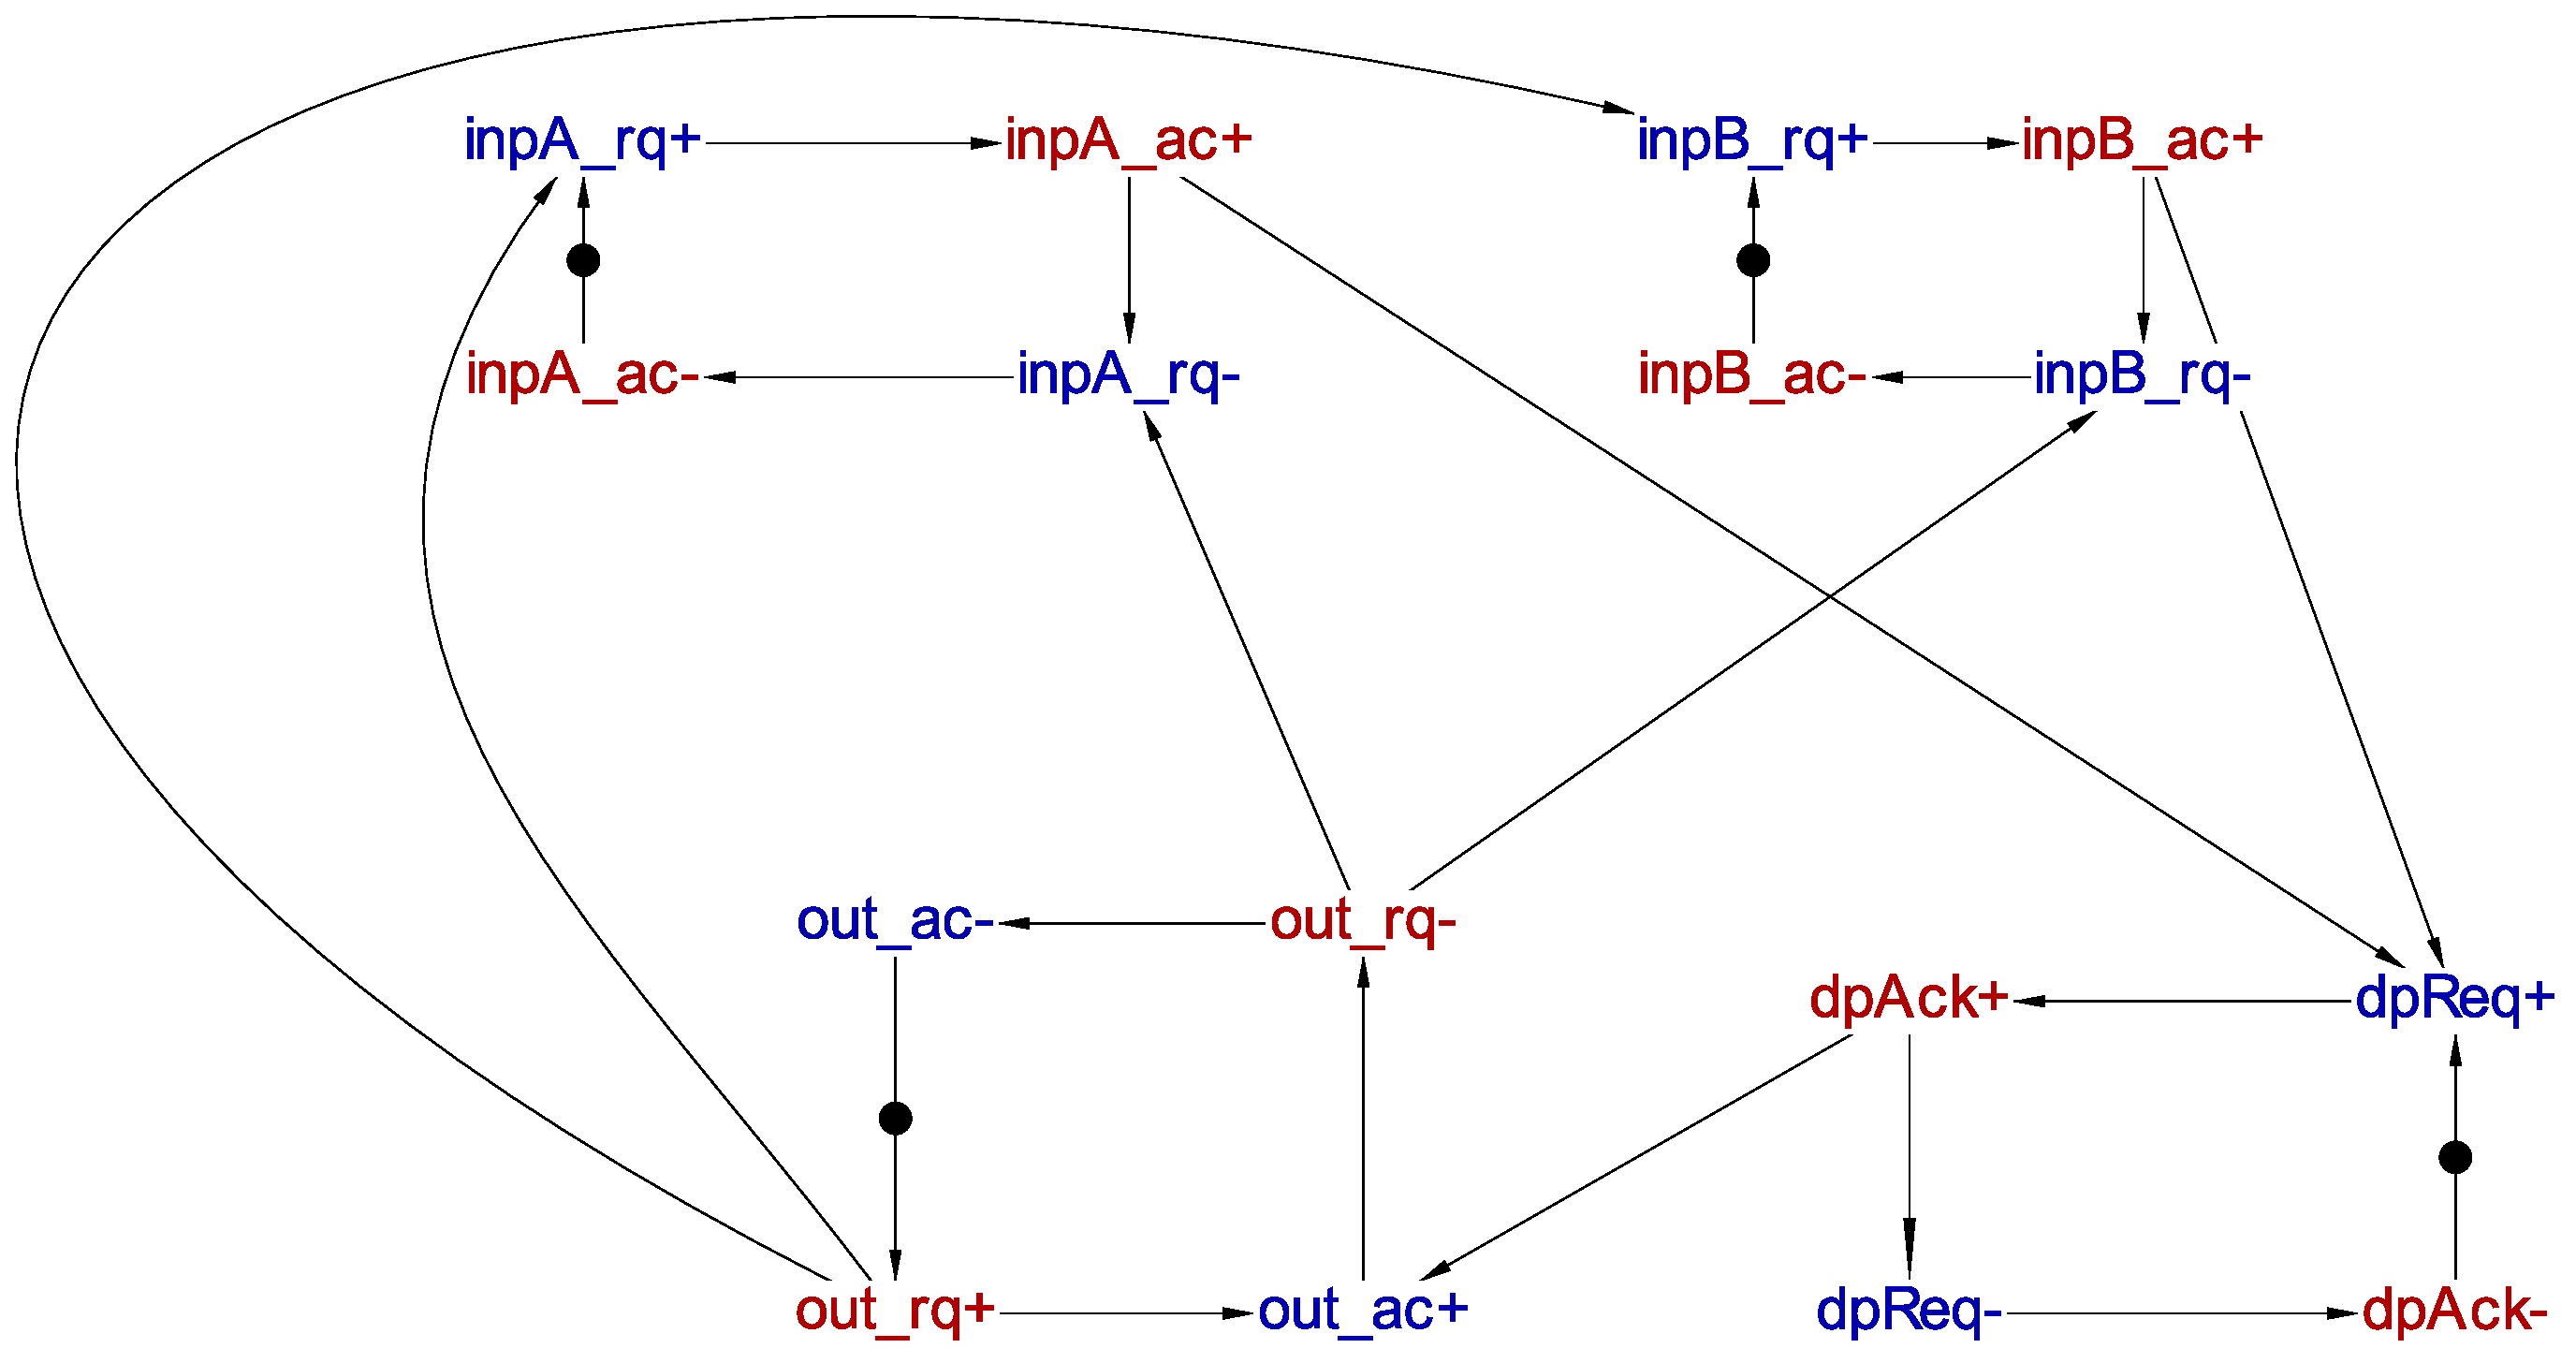
\includegraphics[scale=0.21]{figures/Data/binaryfunc}}
\par\end{centering}
}

\subfloat[CallMux\label{fig:CallMux}]{\begin{centering}
\balsafigSZ{figures/Data/callmux-HC}~~\vcent{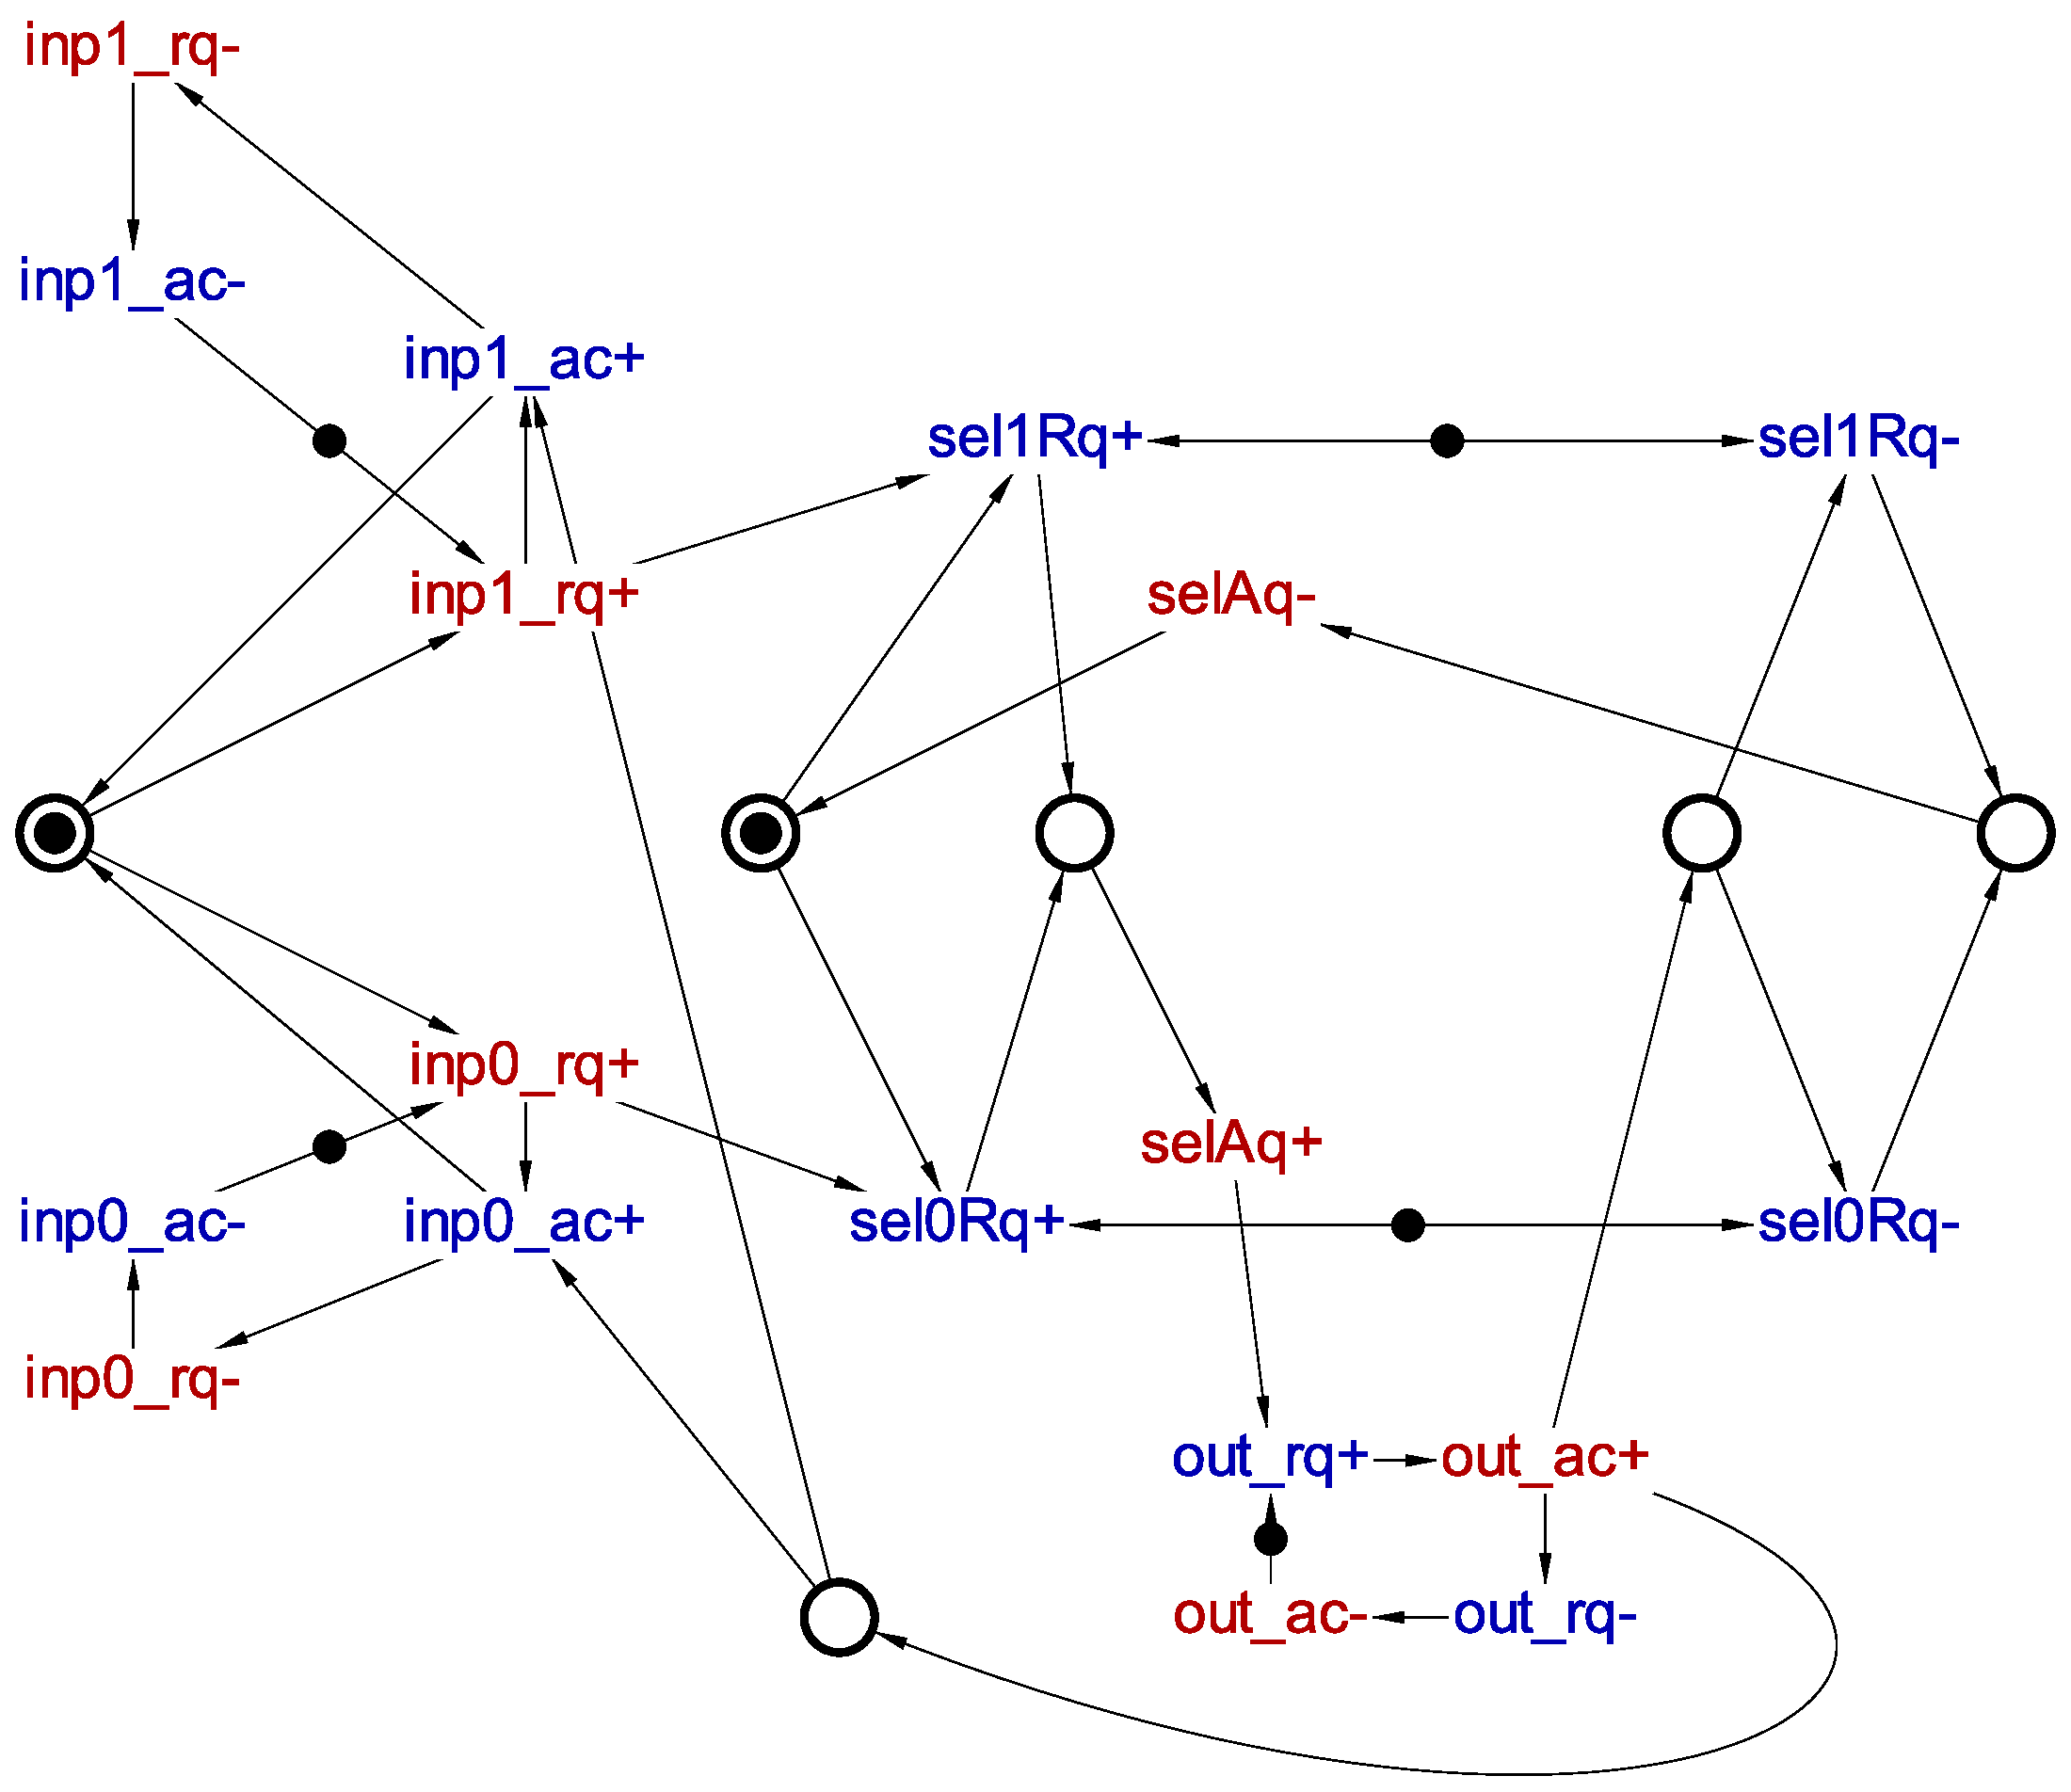
\includegraphics[scale=0.21]{figures/Data/callmux}}
\par\end{centering}
}

\subfloat[Variable\label{fig:Variable}]{\begin{centering}
\balsafigSZ{figures/Data/variable-HC}~~\vcent{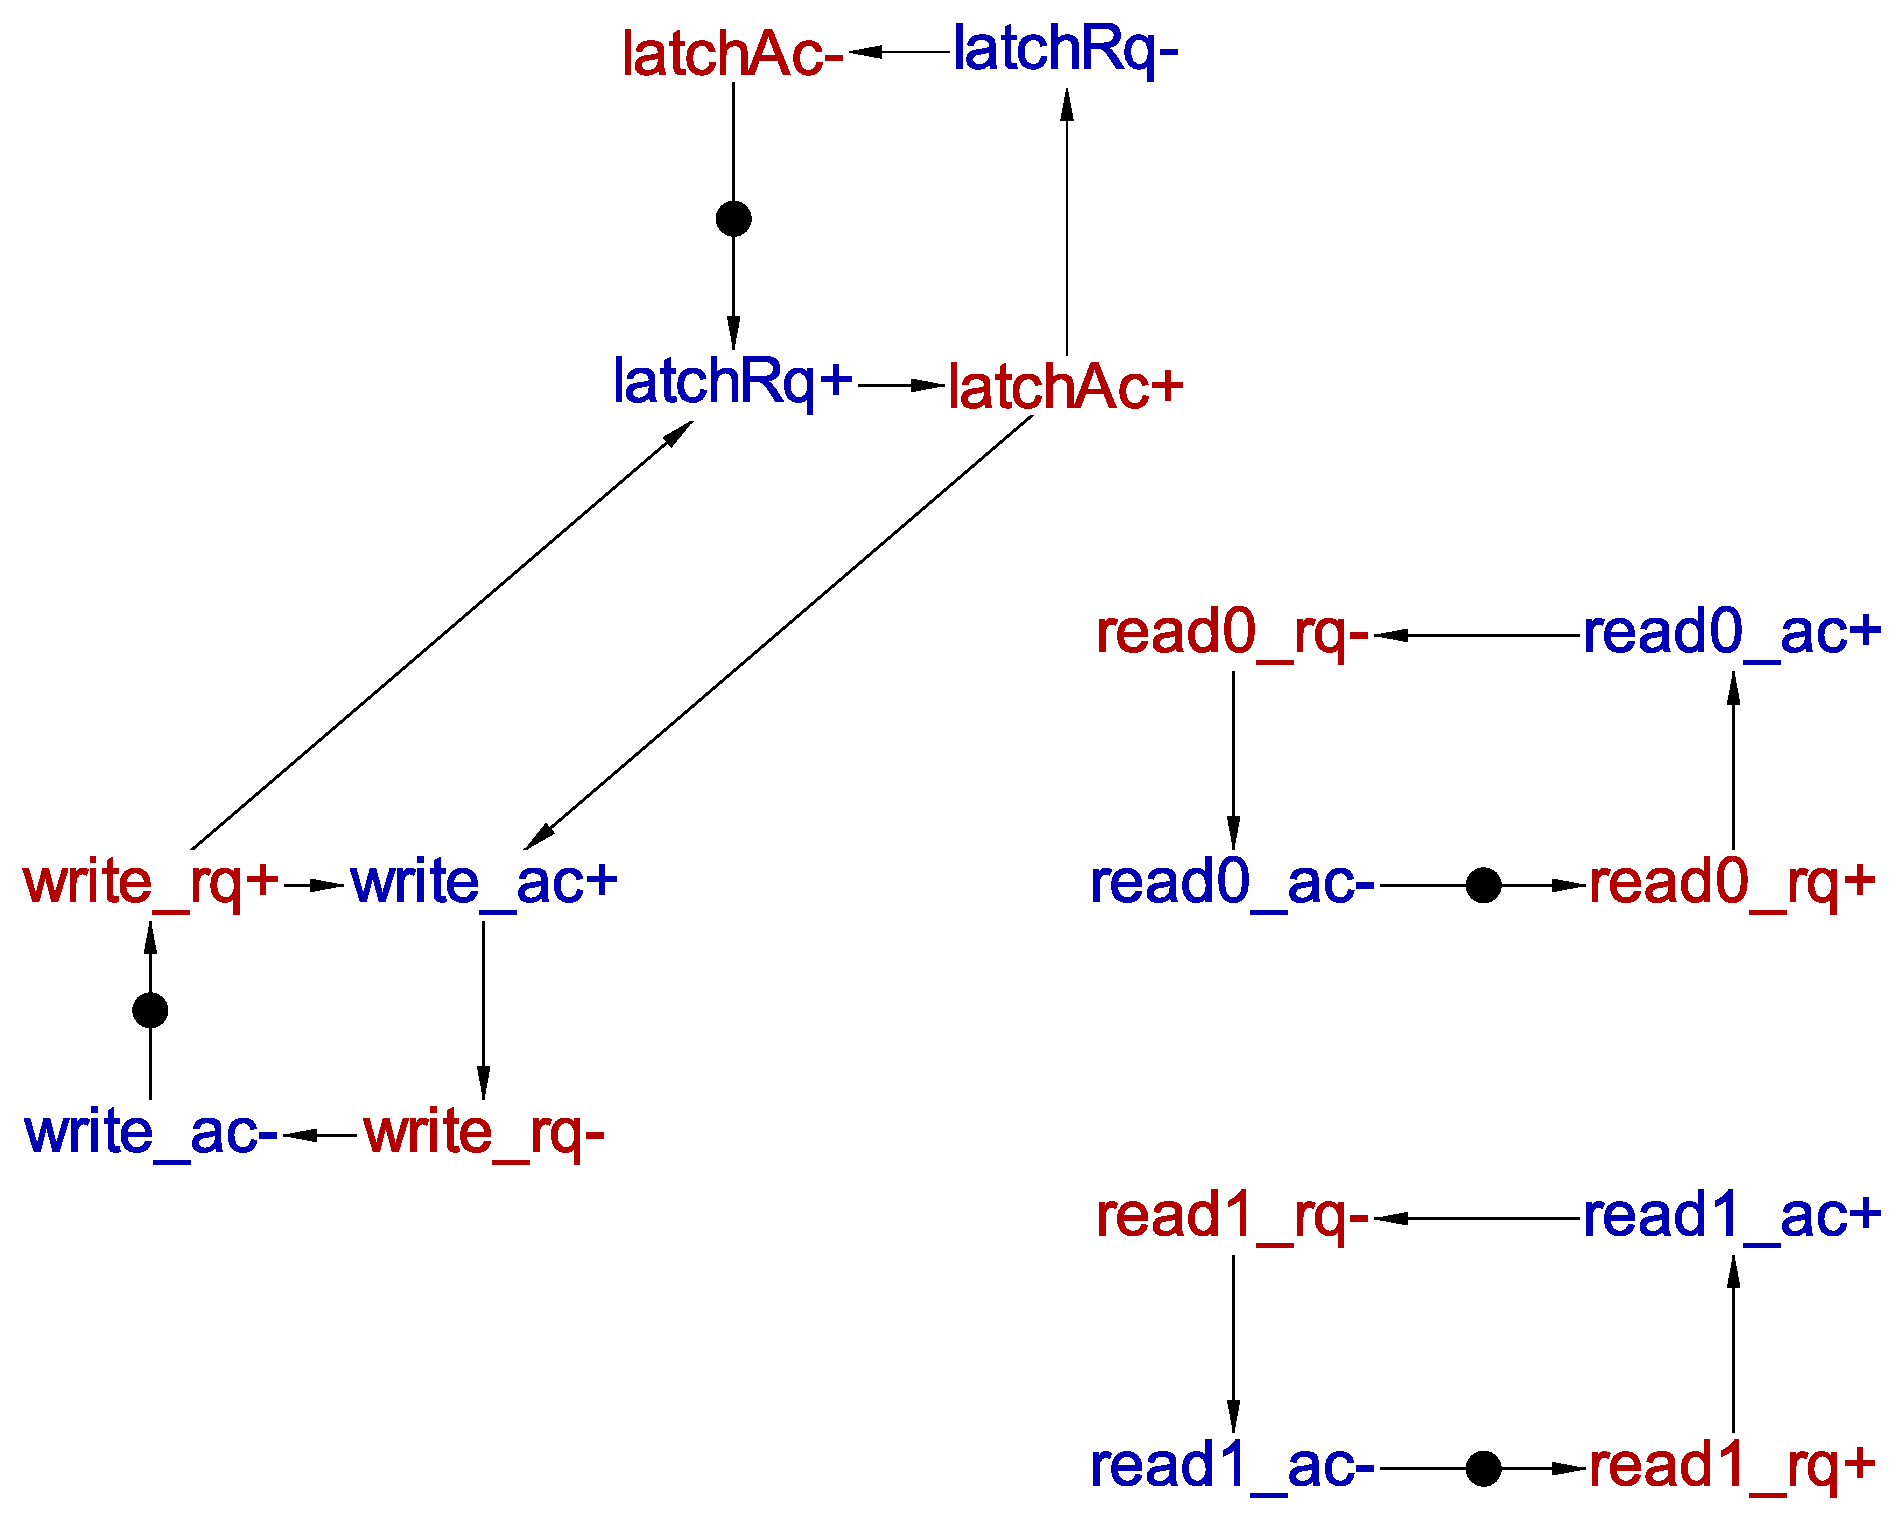
\includegraphics[scale=0.21]{figures/Data/variable}}
\par\end{centering}
}

\caption{Data path control components and their respective STGs}
\end{figure}


This group of components is used to control the the corresponding
data path components that execute predefined operations on data. These
operations are far too complex for automated synthesis, but the control
path part can still be optimised using STG resynthesis, which makes
it reasonable to separate data and control signals. The signals that
control the data path are in this case specified as the input and
output signals of the component's STG. Because the data path blocks
are outside this specification, their handshake protocols must be
implemented strictly and thus cannot be optimised. This, however,
does not prevent the optimisation of handshakes that belong to the
same component but interface with other control path components.

BinaryFunc~(Figure~\ref{fig:BinaryFunc}), CallMux~(Figure~\ref{fig:CallMux}),
Variable~(Figure~\ref{fig:Variable}) are good examples of the data
path control components.


\subsubsection{Data-control interface components}

\begin{figure}
\centering
\begin{raggedright}
\subfloat[While\label{fig:While}]{\begin{centering}
\vcent{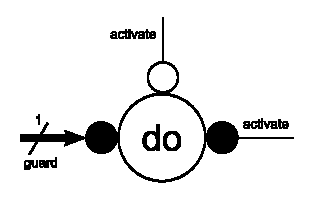
\includegraphics[bb=0bp 0bp 134bp 80bp,scale=0.6]{figures/while-HC}}~~\vcent{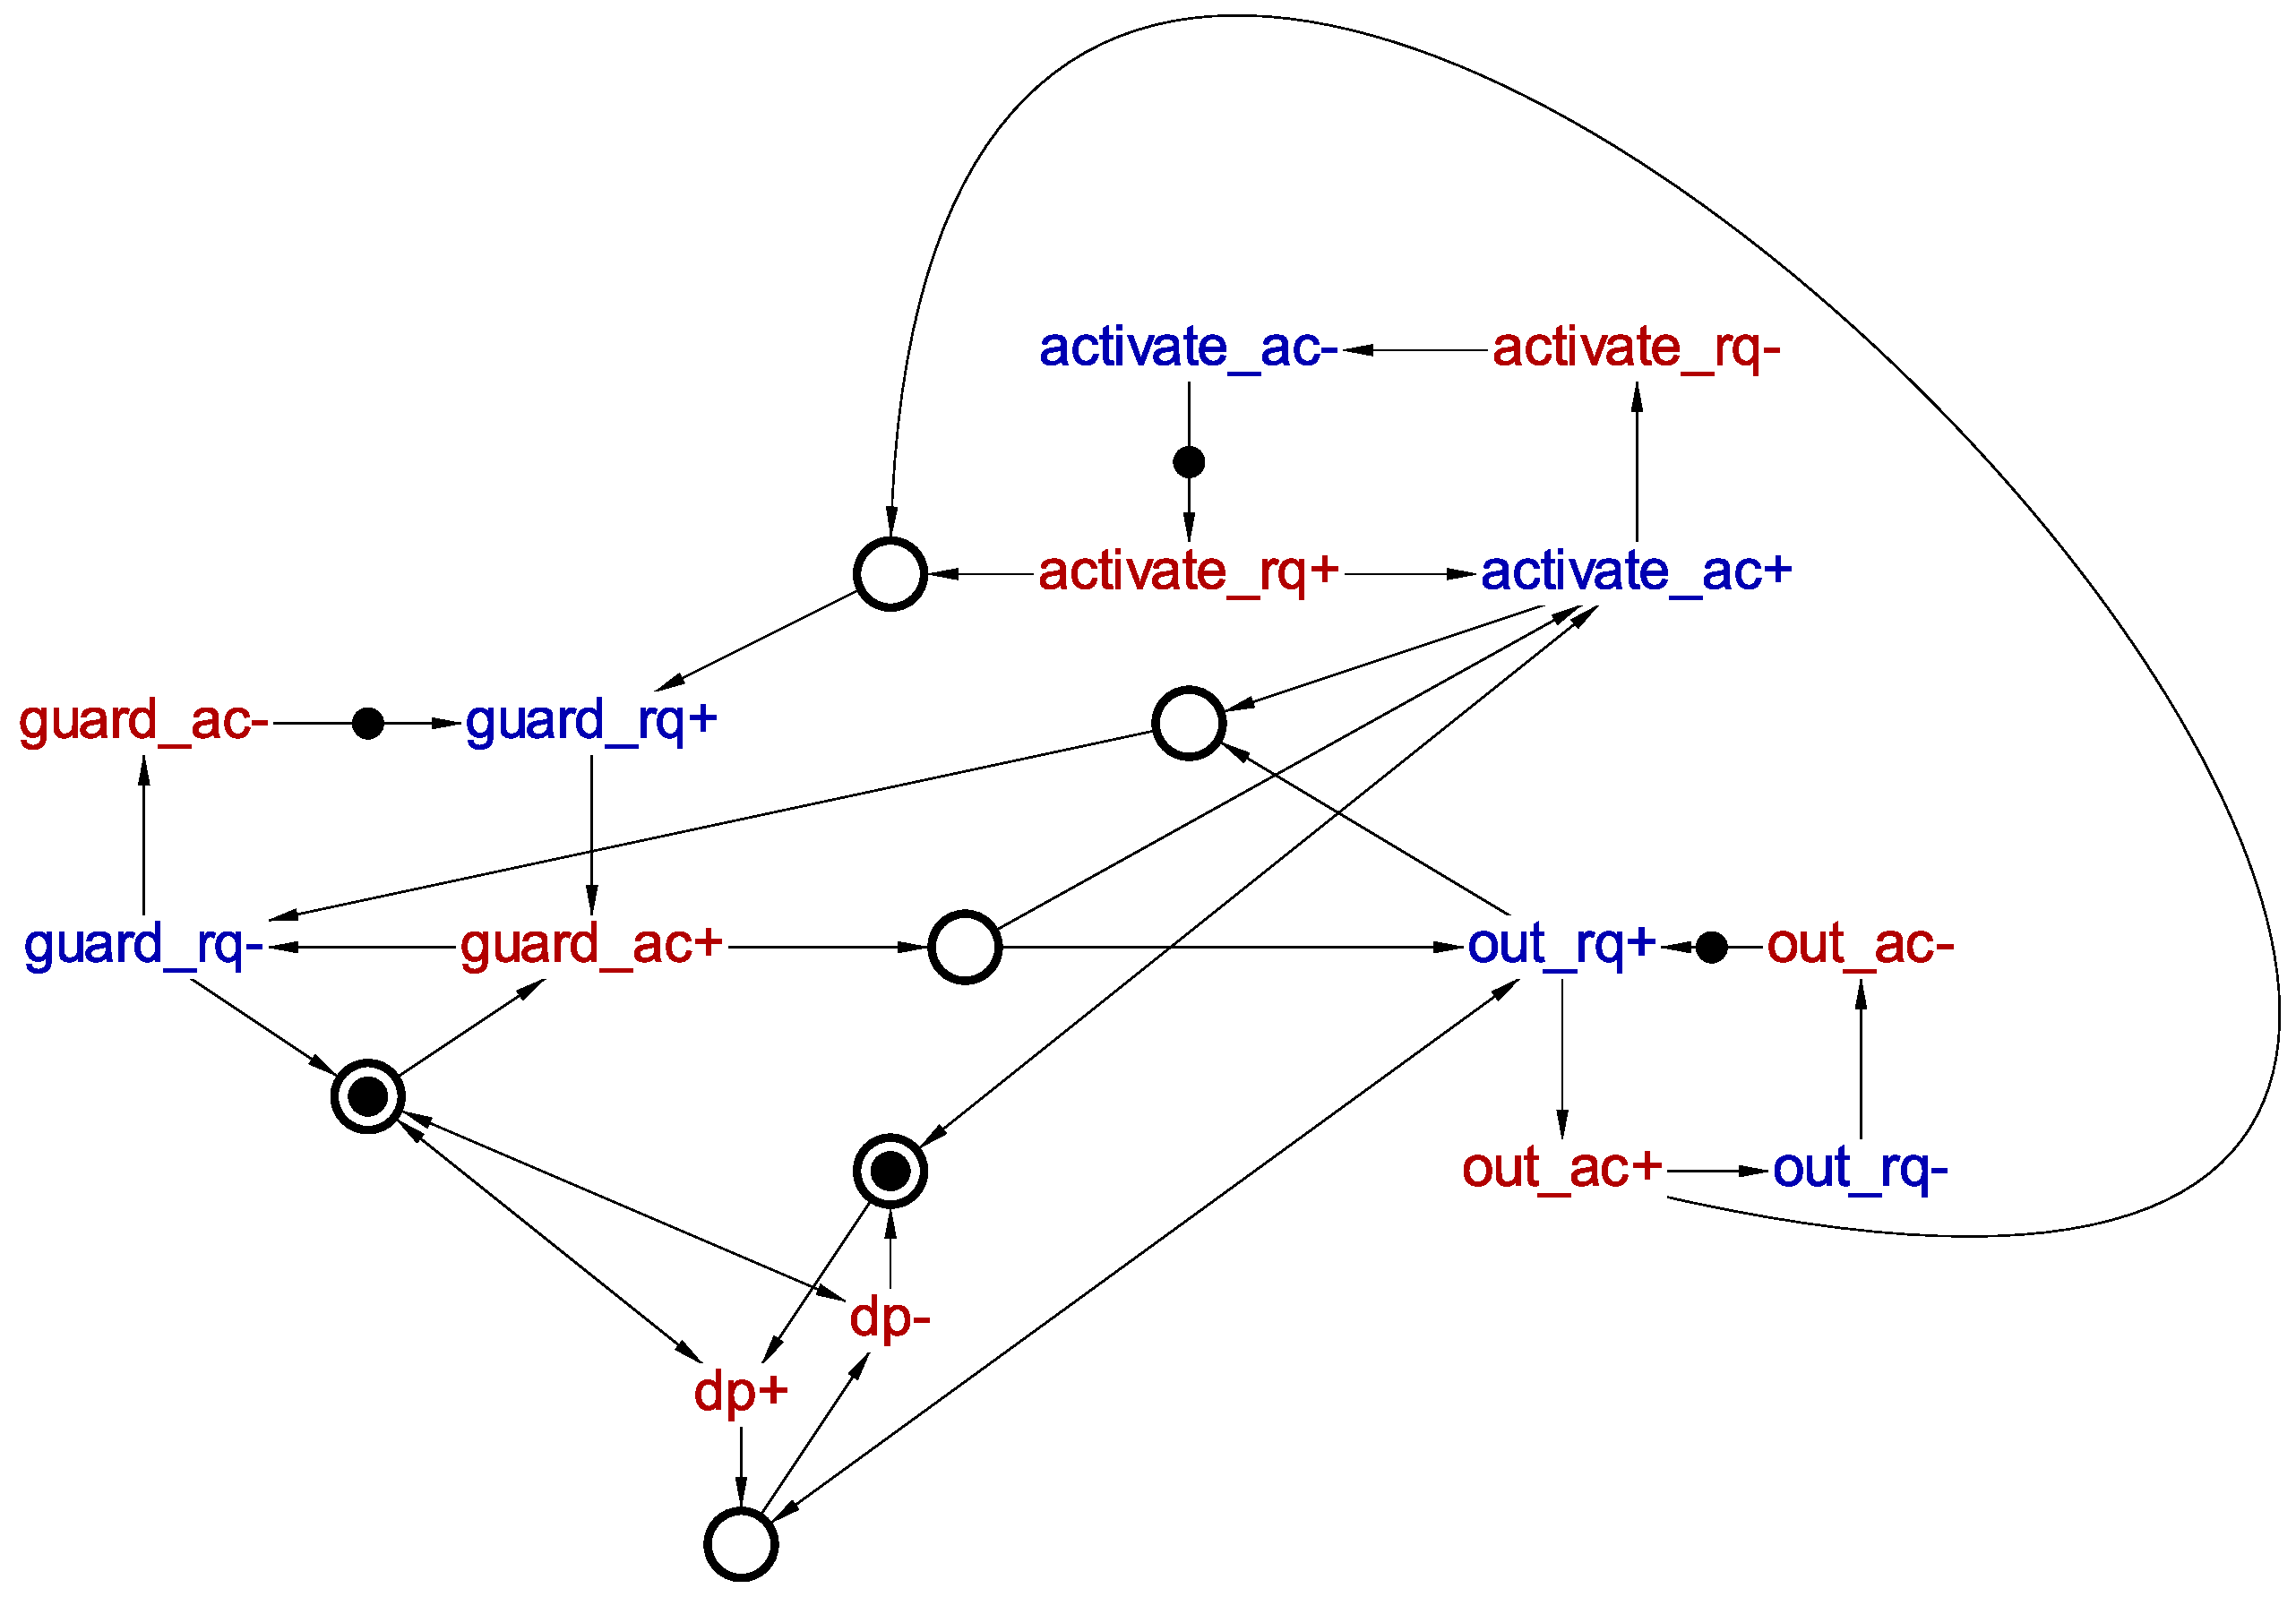
\includegraphics[scale=0.25]{figures/while}}
\par\end{centering}

}
\par\end{raggedright}

\begin{raggedright}
\subfloat[Case\label{fig:Case}]{\begin{centering}
\balsafigSZ{figures/case-HC}~~\vcent{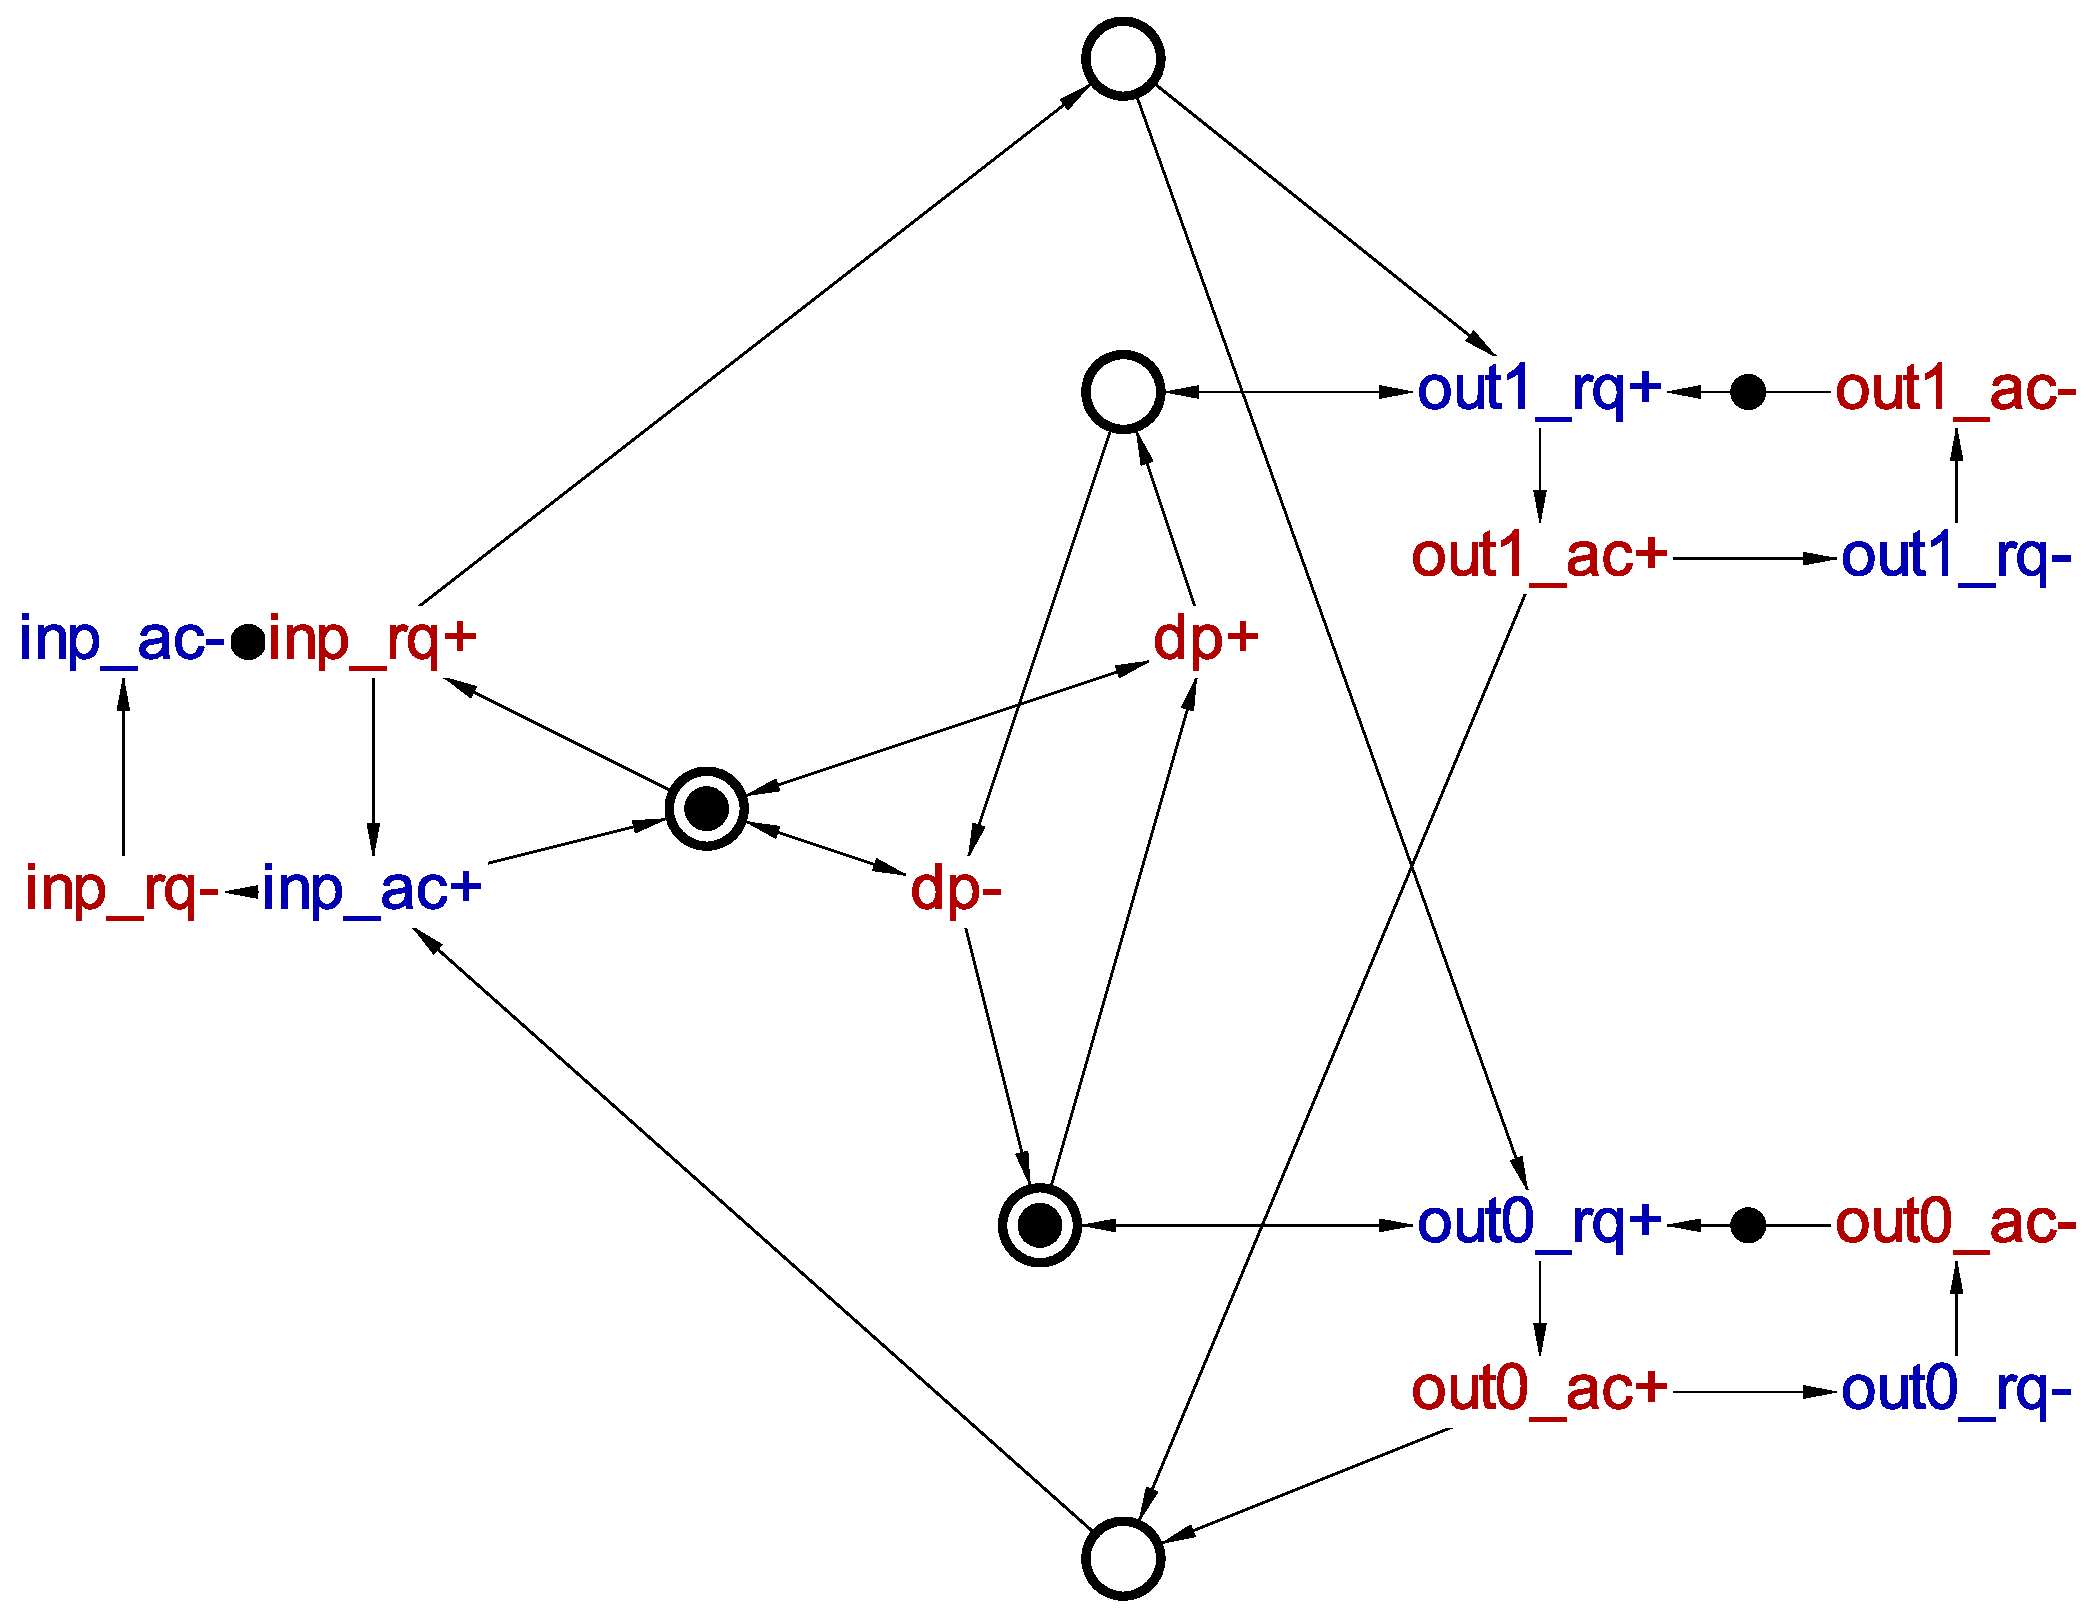
\includegraphics[scale=0.25]{figures/case}}
\par\end{centering}

}
\par\end{raggedright}

\caption{Data-control interface components and their respective STGs\label{fig:Data-control-interface-components}}
\end{figure}


Data-control interface components provide conversion of data to control
signals or vice versa. For example, the While component~(Figure~\ref{fig:While})
analyses the input data to decide whether it should end its operation
and conclude the activation handshake, or to continue activating the
output handshake. Case component~(Figure~\ref{fig:Case}) handles
the data in a very similar way, however it has an arbitrary bus width,
so for bus widths of more than one bit a decoder that resides in the
data path could be used to reduce the STG complexity. These components
STGs can become quite complex and the strict behaviour of their data-path
handshakes must be preserved.


\subsection{An example: GCD controller}

\begin{figure}[!t]
\centering
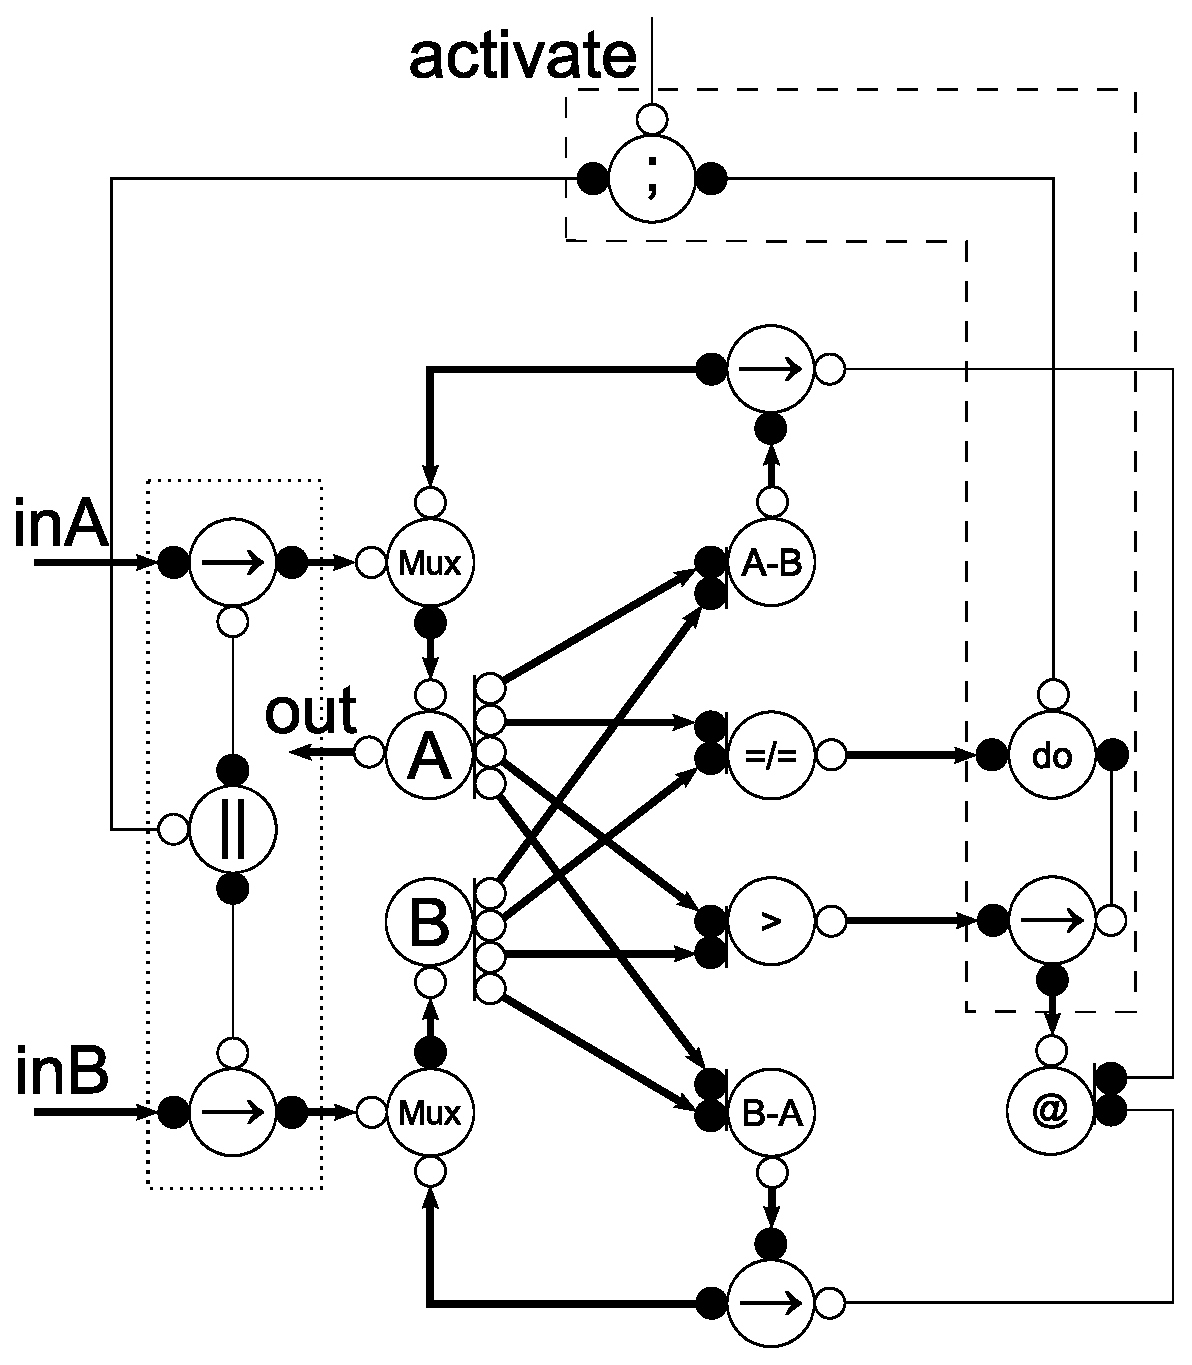
\includegraphics[width=0.3\paperwidth]{figures/breeze-gcd-partition}

\caption{Breeze Handshake Circuit model of a GCD block\label{fig:GCD}}
\end{figure}


We have chosen the GCD controller~(Figure~\ref{fig:GCD}) to demonstrate
how the proposed technique applies to real-life circuits. The GCD
controller is a good research example because it has components from
every group described in section \ref{sec:Individual-component-examples}
and its complexity does not allow omitting of the STG decomposition
step, which is an important part of the proposed workflow. All available
synthesis tools failed to synthesise a circuit from the fully composed
STG model of GCD controller. This proves that the decomposition is
a necessary step lacking which the synthesis of a practical circuit
is not likely to succeed.

Decomposition on the level of STG can be replaced with decomposition
on the level of handshake components. Such decomposition can be done
simply by partitioning the input handshake circuit into blocks, trying
to minimise the number of handshakes between blocks, and applying
the synthesis process to each block separately. While working with
the GCD example it was found that decomposition on the level of handshake
components can be done easier and is guaranteed to be successful,
whereas decomposition on the STG level is a complex task, which requires
additional third-party tools.


\subsection{Experimental results}

\begin{table}[!t]
\begin{centering}
\begin{tabular}{|c|c|c|c|}
\hline 
Component type & \noun{MPSat} cost & \noun{Petrify} cost & Best\tabularnewline
\hline 
\hline 
BinaryFunc & 21 & 27 & 21\tabularnewline
\hline 
Case & 13 & 13 & 13\tabularnewline
\hline 
Fetch & 17 & 13 & 13\tabularnewline
\hline 
Concur & 16 & 16 & 16\tabularnewline
\hline 
Variable & 13 & 18 & 13\tabularnewline
\hline 
Sequence & 13 & 13 & 13\tabularnewline
\hline 
CallMux & 25 & 33 & 25\tabularnewline
\hline 
While & 17 & 17 & 17\tabularnewline
\hline 
\hline 
\noun{Total} & 305 & 333 & 285\tabularnewline
\hline 
\end{tabular}
\par\end{centering}

\caption{Costs of individual components\label{tab:Costs-of-individual}}


\end{table}


\begin{table}[t]
\begin{centering}
\begin{tabular}{|c|c|}
\hline 
\multicolumn{2}{|c|}{\noun{MPSat}}\tabularnewline
\hline 
Synthesised block & Cost\tabularnewline
\hline 
\hline 
seq+concur+2xfetch & 35\tabularnewline
\hline 
fetch+var+2xBF & 49 \tabularnewline
\hline 
fetch+var+2xBF & 49 \tabularnewline
\hline 
fetch+case & 23 \tabularnewline
\hline 
while & 17 \tabularnewline
\hline 
callmux & 25\tabularnewline
\hline 
callmux & 25\tabularnewline
\hline 
\hline 
\noun{Total}  & 223\tabularnewline
\hline 
\end{tabular}\noun{~~~~}%
\begin{tabular}{|c|c|}
\hline 
\multicolumn{2}{|c|}{\noun{Petrify}}\tabularnewline
\hline 
Synthesised block & Cost\tabularnewline
\hline 
\hline 
var+2xBF & 52\tabularnewline
\hline 
var+2xBF & 52\tabularnewline
\hline 
2xfetch+case & 29\tabularnewline
\hline 
fetch+while & 29\tabularnewline
\hline 
seq+concur+fetch & 29\tabularnewline
\hline 
callmux  & 33\tabularnewline
\hline 
fetch & 13\tabularnewline
\hline 
callmux & 33\tabularnewline
\hline 
\hline 
\noun{Total} & 270\tabularnewline
\hline 
\end{tabular}\\
~\\
~\\
~%
\begin{tabular}{|c|c|}
\hline 
\multicolumn{2}{|c|}{\noun{Best choice}}\tabularnewline
\hline 
Synthesised block & Cost\tabularnewline
\hline 
\hline 
var+callmux+2xBF & 63\tabularnewline
\hline 
fetch+while & 29\tabularnewline
\hline 
fetch+case & 21\tabularnewline
\hline 
seq+concur+2xfetch & 35\tabularnewline
\hline 
callmux & 25\tabularnewline
\hline 
fetch+var+2xBF & 47 \tabularnewline
\hline 
\hline 
\noun{Total} & 220\tabularnewline
\hline 
\end{tabular}
\par\end{centering}

\caption{Cost of optimally split full GCD circuit\label{tab:Cost-of-optimally}}


\end{table}


For the evaluation of the proposed method effectiveness, each individual
handshake component was synthesised separately and its cost~(in logic
equation literals) estimated. Then, parts of the GCD handshake circuit
were synthesised from the STG composition, and the cost of this implementation
was compared to the sum of costs of individual components implementations.
For synthesis, two tools were used: MP\noun{Sat} and \noun{Petrify}. 

The process of circuit synthesis using this approach was completely
automated.

In Table~\ref{tab:Costs-of-individual}, the costs of each standalone
handshake component, synthesised from the STG specifications, are
shown. The results are shown for both applied synthesis tools.

In Table~\ref{tab:Cost-of-optimally}, the cost of fully sythesised
GCD controller is shown. The cost was derived for synthesis carried
out by each tool individually, and for the best mix of HC parts produced
by both tools, selected on lowest total cost basis (in Figure~\ref{fig:GCD},
two such parts are highlighted).

It can be seen from the tables that the cost improvement for
the GCD circuit was approximately 28\%.
